\section{Camera Theory}

An image captured through a camera is the result of reflected light being detected on a cameras sensor, see figure \ref{fig:light_cam}. This process is know as \textit{image acquisition}. If you have no previous experience in image processing this might be mumbo-jumbo to you. In this chapter the basics of image acquisition using a digital camera will be explained. To understand this it is necessary to have a rudimentary understanding of the physics behind light.

\begin{figure}[htbp] 
\centering 
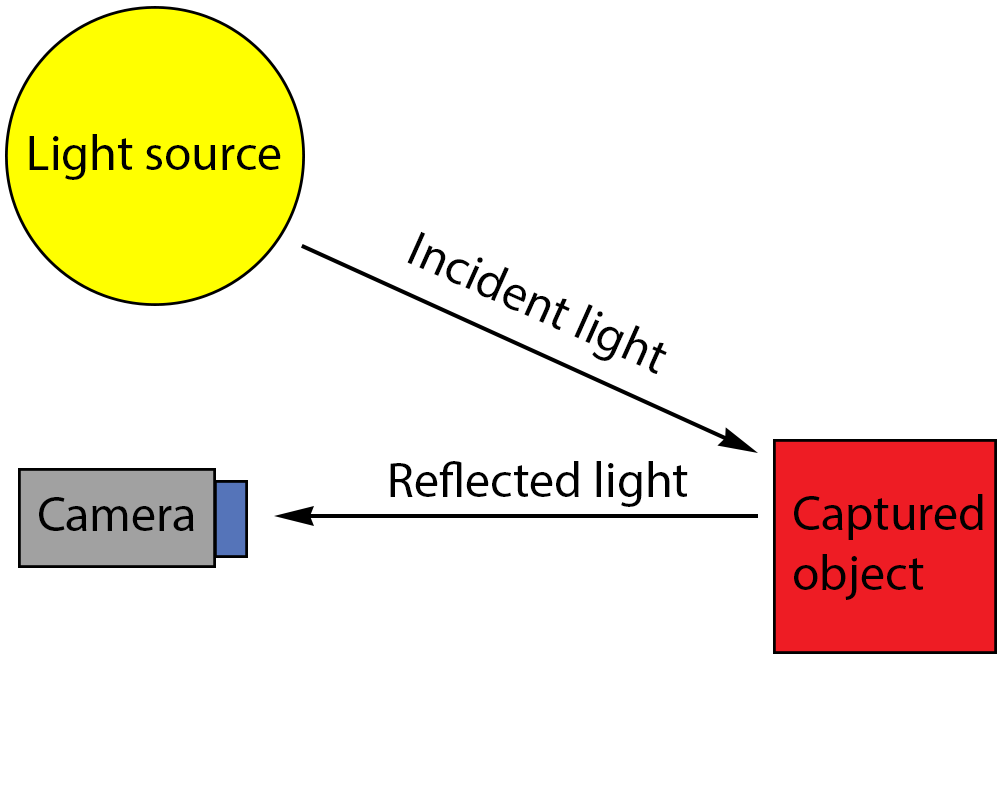
\includegraphics[width=0.5\textwidth]{Pictures/Theory/light_from_sun.png} 
\caption{Light as captured by a camera} 
\label{fig:light_cam} 
\end{figure}

Light is a form of electromagnetic radiation and can be viewed as both waves and particles. This duality is not something that we will be concerned with in this chapter. The wave model is sufficient to build the foundation of our understanding. A light wave is a small packet of energy travelling through space, these energy packet are known as photons. Photons can be described by three properties:

\begin{itemize}
\item \textbf{Wavelenght} - Measured in meters from wave top to wave top and denoted as $\lambda$.
\item \textbf{Frequency} - Measured in oscillations per second, Hz, denoted $f$.
\item \textbf{Energy} - Measured in electronvolts, eV, denoted $E$.
\end{itemize}

The formulae for these properties are as follows:

\begin{align}
\centering 
\lambda = \frac{C}{f}, \text{Where C is the speed of light}
\label{eq:wavelenght} 
\end{align}

\begin{align}
\centering
E = \frac{hC}{\lambda}, \text{Where C is the speed of light}
\label{eq:e_v} 
\end{align}

 


